\documentclass[a4paper,12pt]{article}

\usepackage{latexsym}
\usepackage[utf8]{inputenc}
\usepackage{graphicx}
\usepackage{amsmath}
\usepackage{float}% If comment this, figure moves to Page 2
\usepackage{longtable}
\usepackage{caption}

\author{Krzysztof~Palka and Dominik~Odrowski}
\date{April 11, 2013}

\title{\textsc{Exercise} 348 \\ Hall Effect in P-Germaium} 

\addtolength{\textwidth}{2.5cm}
\addtolength{\hoffset}{-1.25cm}

\begin{document}

\maketitle

    \begin{abstract}
        This report presents examination of Hall effect in the semiconductor, determination od charge carriers, Hall's constant and the mobility and density of carries.         
    \end{abstract}

    \section{Introduction}
    The aim of this exercise was to determine, using sample board, charge carries proprieties and Hall's constant. 

    \section{Theory and measurement}


    If we place conducting flat stripe with steady current $\mathbf{I}$ in a magnetics field $\mathbf{B}$ due to deflection of electrons because of Lorentz force, occurs phenomena called Hall effect. It causes development of the voltage across the sample stripe---Hall voltage $\mathbf{I}$. Knowing direction of current and sense of magnetic field we can determine the polarity of Hall voltage. Figure \ref{fig:set-up} presents the circuit for observation of the Hall effect.

    Hall voltage could be described by equation \ref{eq:Uh}
    \begin{equation}
        U_H = i \cdot \frac{B}{e \cdot d \cdot n} \label{eq:Uh}
    \end{equation}
    where $d$ is thickness, $e$ is electron charge, $B$ is value of magnetic field, $i$ is current and $e$ is the charge carries density.    
    Having this data we can calculate the Hall constant form formula \ref{eq:Ch}
    \begin{equation}
        C_H = \frac{U_H}{B} \cdot \frac{d}{I} = \frac{1}{n \cdot e} \label{eq:Ch}
    \end{equation}

    And having the sample resistance $R$ and sample dimensions $d$, $a$, $l$ we can calculate conductivity $\sigma$:

    \begin{equation}
        \sigma = \frac{l}{R \cdot d \cdot a} \label{eq:sigma}
    \end{equation}

    The, when we know value of sigma we can substitute it to equation for carries mobility $\mu_H$

    \begin{equation}
        \mu_H = C_H \cdot \sigma \label{eq:mu} 
    \end{equation}
    
    We can determinate polarity of Hall voltage using sign of the charge carries.
    
    For experiment we would use set-up shown on figure \ref{fig:set-up} 

    \begin{figure}[H]
    \begin{center}
        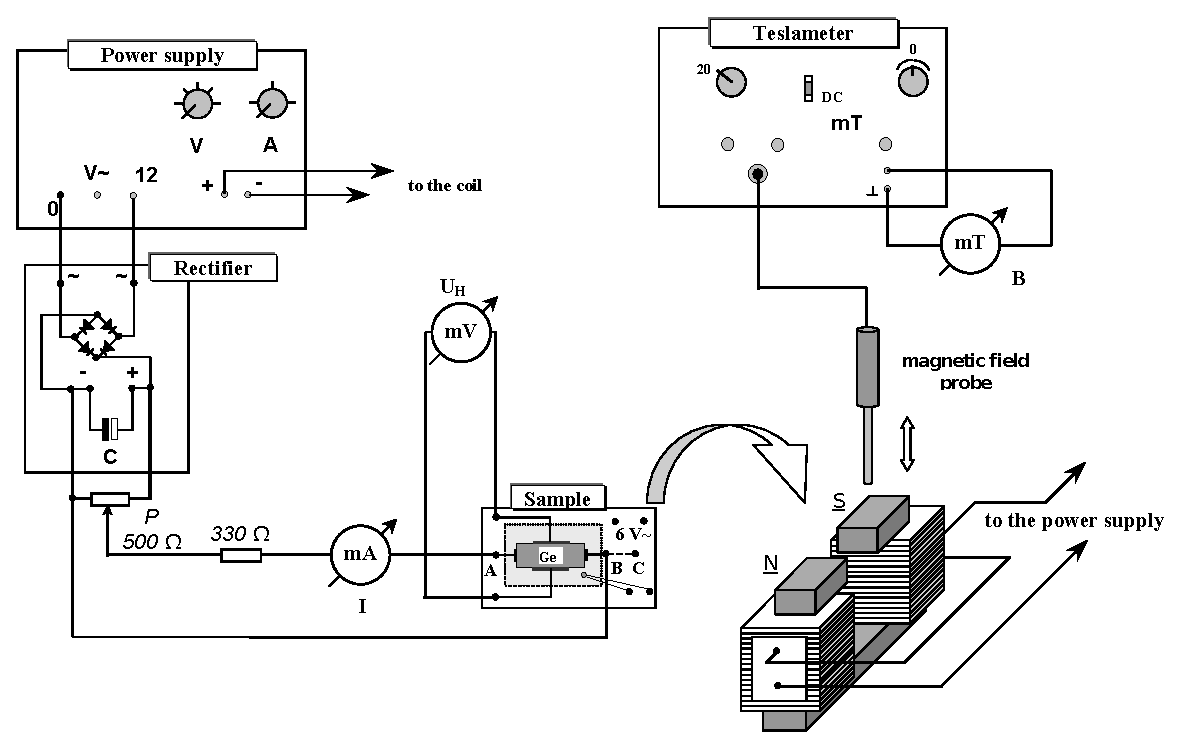
\includegraphics[width=0.8\textwidth]{set-up}
        \caption{Diagram of experimental set-up \cite{E22}. It consists of teslameter, power supply, rectifier, sample of examined material and magnetic probe.}
        \label{fig:set-up}
    \end{center}
    \end{figure}

    \section{Results}
    Firstly we have measured the Hall voltage $U_H$ depending on current $I$ through the sample, the Hall voltage depending on strength of magnetic field $B$.
    
    \begin{table}[H]
    \begin{minipage}[t]{.40\textwidth}
      \centering
      \begin{tabular}{ | c | c |}
        \hline
        I [mA] & $\mathrm{U_H}$ [mV] \\ \hline
        \hline
        -58 & 103.7\\
        -53 & 95.9\\
        -50 & 88.3\\
        -45 & 81.7\\
        -40 & 70.8\\
        -35 & 63.1\\
        -30 & 55.5\\
        -25 & 47.3\\
        -20 & 37.9\\
        -15 & 29.8\\
        -10 & 21.5\\
        -5 & 13.0\\
        0 & 1.7\\
        5 & -6.5\\
        10 & -15.3\\
        15 & -24.8\\
        20 & -33.5\\
        25 & -40.8\\
        30 & -50.1\\
        35 & -57.2\\
        40 & -67.2\\
        45 & -73.6\\
        50 & -82.0\\
        55 & -90.7\\
        60 & -98.6\\
        61 & -101.4\\ \hline
      \end{tabular}
      \caption{Graph of Hall voltage depending on current through sample with constant magnetic field field $B$ = 300 mT}
    \end{minipage}\qquad
    \begin{minipage}[t]{.40\textwidth}
      \centering
      \begin{tabular}{ | c | c || c | c |}
        \hline
        B [mT] & $\mathrm{U_H}$ [mV] & B [mT] & $\mathrm{U_H}$ [mV]\\ \hline

            -406 & 68.7 & 0 & 3.8\\
            -400 & 67.7 & 20 & -1.2\\
            -380 & 64.6 & 40 & -4.6\\
            -360 & 61.5 & 60 & -8.0\\
            -340 & 58.3 & 80 & -11.3\\
            -320 & 55.1 & 100 & -14.7\\
            -300 & 52.0 & 120 & -18.2\\
            -280 & 48.8 & 140 & -21.7\\
            -260 & 45.5 & 160 & -25.1\\
            -240 & 42.4 & 180 & -28.5\\
            -220 & 39.1 & 200 & -32.0\\
            -200 & 35.8 & 220 & -35.4\\
            -180 & 32.5 & 240 & -38.7\\
            -160 & 29.2 & 260 & -42.3\\
            -140 & 26.0 & 280 & -45.6\\
            -120 & 22.7 & 300 & -49.1\\
            -100 & 19.0 & 320 & -52.5\\
            -80 & 16.0 & 340 & -55.9\\
            -60 & 16.0 & 360 & -59.4\\
            -40 & 12.6 & 380 & -62.7\\
            -20 & 9.3 & 400 & -66.2\\
            -8 & 5.8 & 405 & -66.9\\

      \hline
      \end{tabular}
      \caption{Hall voltage depending on strength of magnetic field for constant current $I_P$~=~30 mA}
    \end{minipage}
    \end{table}

    After mark measured points on plot we can observe, that linearity of results is almost fulfilled.

    \begin{figure}[H]
        \begin{center}
            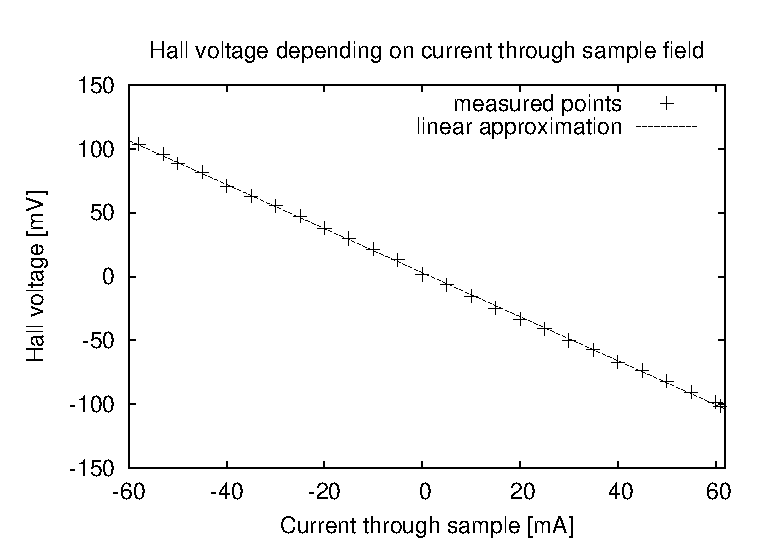
\includegraphics[width=0.70\textwidth]{U_H-vs-I_P}
            \caption{Graph of Hall voltage depending on current through sample with constant magnetic field field $B$~=~300 mT}
            \label{fig:U_H-vs-I_P}
        \end{center}
    \end{figure}

    \begin{figure}[H]
        \begin{center}
            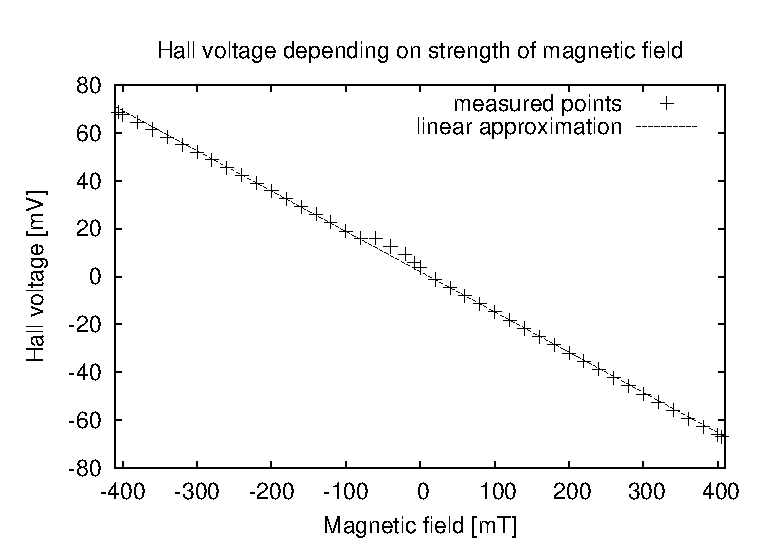
\includegraphics[width=0.70\textwidth]{U_H-vs-B}
            \caption{Graph of Hall voltage depending on strength of magnetic field for constant current $I_P$ = 30 mA}
            \label{fig:U_H-vs-B}
        \end{center}
    \end{figure}

    From linear regression for slope $R_H$ for figure \ref{fig:U_H-vs-I_P} we have got $R_H = (-1.725 \pm 0.006) \mathrm{\Omega}$. And for fig. \ref{fig:U_H-vs-B}, using the same method of finding slope, $b = (-0.1683 \pm 0.0008) \frac{\mathrm{V}}{\mathrm{T}}$

    Hence $b = \frac{U_H}{B}$ we can substitute it to eq. \ref{eq:Ch} and obtain
    \begin{equation}
        C_H = b \cdot \frac{d}{I}
    \end{equation}
    Now, we substituting obtained data and given $d = 10^{-3}$ m
    \begin{displaymath}
        C_H = -1.68 \cdot 10^{-1} \frac{\mathrm{V}}{\mathrm{T}} \cdot \frac{10^{-3} \mathrm{m}}{-3 \cdot 10^{-2} \mathrm{A}} = 5.600 \cdot 10^{-1} \frac{\mathrm{\Omega m}}{\mathrm{T}}
    \end{displaymath}

    Calculation of propagation of uncertainty

    \begin{equation}
        \Delta C_H = \frac{d}{I} \cdot \Delta b
    \end{equation}
    
    \begin{displaymath}
        \Delta C_H = \frac{10^{-3}\mathrm{m}}{3 \cdot 10^{-2} \mathrm{A}} \cdot 0.0008 \frac{\mathrm{U_H}}{\mathrm{B}} < 0.001 \frac{\mathrm{\Omega m}}{\mathrm{T}}
    \end{displaymath}

    Substituting given data ($l = 2 \cdot 10^{-2}$ m, $a = 5 \cdot 10^{-3}$ m and $R = 57 \, \Omega$) to eq. \ref{eq:sigma}

    \begin{displaymath}
        \sigma = \frac{2 \cdot 10^{-2} \mathrm{m}}{57 \mathrm{\Omega} \cdot 10^{-3} \mathrm{m} \cdot 5 \cdot 10^{-3} \mathrm{m}} = 7.018 \cdot 10^4 \frac{1}{\mathrm{\Omega m}}
    \end{displaymath}

    And according to eq. \ref{eq:mu}

    \begin{displaymath}
        \mu_H =  5.60 \cdot 10^{-1} \frac{\mathrm{\Omega m}}{\mathrm{T}} \cdot 7.01 \cdot 10^4 \frac{1}{\mathrm{\Omega m}} = 3.930 \cdot 10^{-2} \frac{1}{\mathrm{T}}
    \end{displaymath}
    
    \section{Conclusions}
    Despite quite big Asymptotic Standard Error of y-intercept---$\pm$ 0.1955 (9.463\%) during calculation of equation of $B(U_H)$ function, we have obtained very small ASP of slope---$\pm$ 0.0008003 (0.4754\%), and the second results was necessary for further calculation. Thanks to that we got uncertainty less than resolution of results, so we have skipped it. In p-type semiconductor we observe lack of electrons, ``Empty fields'' called ``holes'' are treated as positive charges. When electron move from one hole to another it make effect of reversed polarity. Due to bigger effective mass of holes than electrons, conductivity of this type of semiconductor is less then conductivity of n-type semiconductors. 



    \begin{thebibliography}{9}
    \bibitem{E22}\emph{Experiment 22. Hall Effect in P-Germanium} (2005) [online]. Bogdan Żółtowski. Łódź. Available online at: http://phys.p.lodz.pl/materialy/mdems/348.pdf Accessed April 11, 2013.
        \bibitem{HRW}\emph{Fundamentals of physics} (2011) [ebook]. David Halliday, Robert Resnick, Jearl Walker. 9th ed. ISBN 978-0-470-46908-8
    \end{thebibliography}
\end{document}
